The current document describes the testing procedures adopted in 
the development of the hazard component of the \gls{acr:oqe}, the 
open source hazard and risk software developed by the Global 
Earthquake Model initiative.

Nowadays seismic hazard analysis serves different needs coming 
from a variety of users and applications.
%
These may encompass engineering design, assessment of earthquake risk 
to portfolios of assets within the insurance and reinsurance sectors, 
engineering seismological research, and effective mitigation via public 
policy in the form of urban zoning and building design code formulation.

Decisions based on seismic risk results may have impacts on
population, properties and capitals, possibly with important repercussions 
on our day-to-day life. For these reasons, it is recommendable that 
the generation of hazard models and their calculation is based on 
well-recognized, state-of-the-art and tested techniques, requirements 
that must be reconciled with the need to regularly incorporate 
recent advances given the progress carried out within the 
scientific community.
%
The features described below contribute to fulfill these requirements: 
%
\begin{itemize}
    \item Software should have a modular and flexible structure capable of 
    incorporating new features and - as a consequence - offer users 
    the most recent and advanced techniques.
    %
    In very general terms, modularity is the level to which a component 
    of a system can be moved, replaced or reused.
    %
    In software design, modularity means the separation of the software
    into smaller independent components that can be implemented, maintained 
    and tested easily and efficiently.
    %
    \item Software should have and extensive test coverage which captures 
    possible errors and avoids regressions (i.e. unexpected behaviors 
    introduced by new features).
    %
    Software testing \parencite{myers2012} is an important, complex and 
    vast discipline which helps in developing methods and processes aimed at 
    certifying the extent to which a computer code behaves according 
    to the original design intent and user specifications.
\end{itemize}
% . . . . . . . . . . . . . . . . . . . . . . . . . . . . . . . . . . . > Figure
\begin{figure}[!ht]
\centering
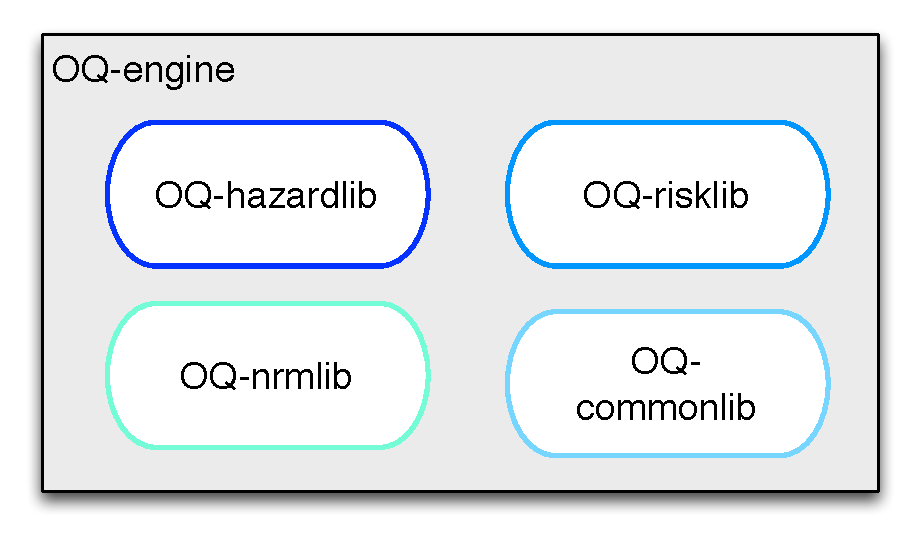
\includegraphics[width=9cm]{figures/oq-engine_structure.pdf}
\caption{A schematic describing the main components of the OpenQuake-engine 
    software.}
\label{fig:oqe_structure}
\end{figure}
% . . . . . . . . . . . . . . . . . . . . . . . . . . . . . . . . . . . < Figure
%
The \gls{acr:oqe} includes different levels of modularity. 
The first is the one separating the engine itself into a number of 
libraries (see Figure \ref{fig:oqe_structure}), each one containing well 
identified knowledge, objects and methods (e.g. the OQ-hazardlib  
includes objects and methods needed to compute probabilistic 
seismic hazard and the OQ-risklib contains methods to compute scenario 
and probabilistic seismic risk).
%
The second one pertains to the data model adopted in the development 
of each library as a result of the abstraction process.
%
According to \textcite{berkes2012} scientific software must be:
\begin{itemize}
\item Error proof
\item Flexible and able to accommodate different methods
\item Reproducible and re-usable
\end{itemize}
%
% ..............................................................................
\section{Testing and Quality Assurance}
Despite the distinction between software testing (in some cases also called 
Quality Control) and \gls{acr:sqa} being somewhat vague and partly open to personal 
judgment, it's clear that \gls{acr:sqa} is a more comprehensive and 
overarching process than software testing.
%
\gls{acr:sqa} aims at the definition of the best processes  
that should be used to provide guarantees that user expectations will 
be met.
%
Software testing focuses instead on detecting software faults by inspecting 
and testing the product at different stages of development.
%
% . . . . . . . . . . . . . . . . . . . . . . . . . . . . . . . . . . . . . . .
\subsection{Testing}
Software testing can be implemented at different stages of the development 
process, with varying strategies to approach the problem.
%
The \gls{acr:oqe} and the associated libraries are developed following an 
agile paradigm. This development strategy is organized in a way that 
the creation of the real code is completed in parallel and fully 
integrated with the software testing process.

The software engineering community provides a wide range of testing levels
and typologies. In the current document we consider just a portion of them
with the specific intent to illustrate the standards used in the 
development of the \gls{acr:oqe} and particularly of its hazard component.
%
% . . . . . . . . . . . . . . . . . . . . . . . . . . . . . . . . . . . . . . .
\subsection{Quality Assurance}
From the IEEE ``Standard for Software Quality Assurance Processes'':
\emph{Software quality assurance is a set of activities that define and 
assess the adequacy of software processes to provide evidence that establishes 
confidence that the software processes are appropriate for and produce 
software products of suitable quality for their intended purposes. 
A key attribute of SQA is the objectivity of the SQA function with 
respect to the project. The SQA function may also be organizationally 
independent of the project; that is, free from technical, managerial, 
and financial pressures from the project.} In this document we are not 
covering topics related to \gls{acr:sqa} since this would go beyond its
scopes.
%
% ..............................................................................
\section{Document structure}
The document is organized into four main chapters and two appendixes.

In the current chapter we provide a very brief and general introduction 
to software testing with a focus on the testing of scientific software. 

In the second chapter we describe the module, or unit, testing, 
the acceptance tests adopted in the development of the 
\gls{acr:oqe} and we discuss some examples.

In the third and fourth chapters we illustrate tests comparing 
the results computed with the \gls{acr:oqe} against the ones 
computed using different probabilistic seismic hazard analysis 
software.

Appendix \ref{sec:app1} provides details on the PEER tests 
implemented in the \gls{acr:oqhl}.
